\textbf{Contributions}

This chapter expands on work presented in

~\autocite{hodsonOnedimensionalLongrangeFalikovKimball2021} \href{https://link.aps.org/doi/10.1103/PhysRevB.104.045116}{One-dimensional long-range Falikov-Kimball model: Thermal phase transition and disorder-free localization}, Hodson, T. and Willsher, J. and Knolle, J., Phys. Rev.~B, \textbf{104}, 4, 2021,

The code is available online~\autocite{hodsonMCMCFKModel2021}.

Johannes had the initial idea to use a long range Ising term to stabilise order in a one dimension Falicov-Kimball model. Josef developed a proof of concept during a summer project at Imperial along with Alexander Belcik. I wrote the simulation code and performed all the analysis presented here.

\textbf{Chapter Summary}

The paper is organised as follows. First, I will introduce the long range Falicov-Kimball (LRFK) model and motivate its definition. Second, I will present the~\protect\hyperlink{sec:lrfk-methods}{methods} used to solve it numerically, including Markov chain Monte Carlo and finite size scaling. I will then present and interpret the~\protect\hyperlink{sec:lrfk-results}{results} obtained.

\hypertarget{sec:lrfk-model}{%
\section{The Model}\label{sec:lrfk-model}}

Dimensionality is crucial for the physics of both localisation and phase transitions. We have already seen that the one dimensional standard FK model cannot support an ordered phase at finite temperatures and therefore has no finite temperature phase transition (FTPT).

On bipartite lattices in dimensions 2 and above the FK model exhibits a finite temperature phase transition to an ordered charge density wave (CDW) phase~\autocite{maskaThermodynamicsTwodimensionalFalicovKimball2006}. In this phase, the spins order anti-ferromagnetically, breaking the \(\mathbb{Z}_2\) symmetry. In 1D, however, Peierls's argument~\autocite{peierlsIsingModelFerromagnetism1936,kennedyItinerantElectronModel1986} states that domain walls only introduce a constant energy penalty into the free energy while bringing a entropic contribution logarithmic in system size. Hence the 1D model does not have a finite temperature phase transition. However 1D systems are much easier to study numerically and admit simpler realisations experimentally. We therefore introduce a long-range coupling between the ions in order to stabilise a CDW phase in 1D.

\hypertarget{fig:lrfk_schematic}{%
\begin{figure}
\centering
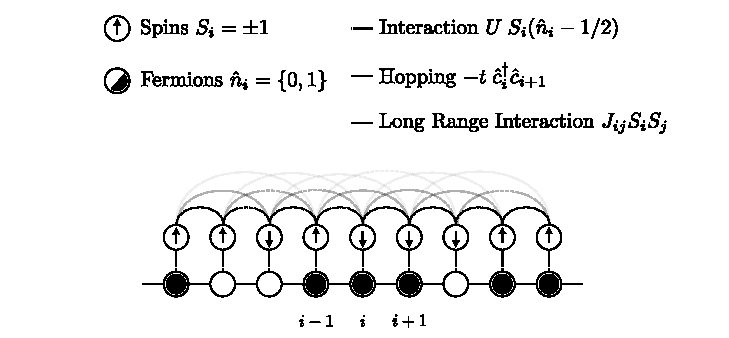
\includegraphics[width=1\textwidth,height=\textheight]{figure_code/intro_chapter/lrfk_schematic}
\caption[{Falicov-Kimball Model Diagram}]{The Long Range Falicov-Kimball (LRFK) Model is a model of classical spins \(S_i\) coupled to spinless fermions \(\hat{c}_i\) where the fermions are mobile with hopping \(t\) and the fermions are coupled to the spins by an Ising type interaction with strength \(U\). The difference from the standard FK model is the presence of a long range interaction between the spins \(J_{ij}S_i S_j\).}
\label{fig:lrfk_schematic}
\end{figure}
}

We interpret the FK model as a model of spinless fermions, \(c^\dagger_{i}\), hopping on a 1D lattice against a classical Ising spin background, \(S_i \in {\pm \frac{1}{2}}\). The fermions couple to the spins via an onsite interaction with strength \(U\) which we supplement by a long-range interaction, \[
J_{ij} = 4\kappa J\; (-1)^{|i-j|} |i-j|^{-\alpha},
\]

between the spins. The additional coupling is very similar to that of the long range Ising model, it stabilises the Antiferromagnetic (AFM) order of the Ising spins which promotes the finite temperature CDW phase of the fermionic sector.

The hopping strength of the electrons, \(t = 1\), sets the overall energy scale and we concentrate throughout on the particle-hole symmetric point at zero chemical potential and half filling~\autocite{gruberFalicovKimballModelReview1996}.

\[\begin{aligned}
H_{\mathrm{FK}} = & \;U \sum_{i} S_i\;(c^\dagger_{i}c_{i} - \tfrac{1}{2}) -\;t \sum_{i} (c^\dagger_{i}c_{i+1} + \textit{h.c.)}\\ 
 &  + \sum_{i, j}^{N} J_{ij}  S_i S_j
\label{eq:HFK}\end{aligned}\]

Without proper normalisation, the long range coupling would render the critical temperature strongly system size dependent for small system sizes. Within a mean field approximation the critical temperature scales with the effective coupling to all the neighbours of each site, which for a system with \(N\) sites is \(\sum_{i=1}^{N} i^{-\alpha}\). Hence, the normalisation \(\kappa^{-1} = \sum_{i=1}^{N} i^{-\alpha}\), renders the critical temperature independent of system size in the mean field approximation. This greatly improves the finite size behaviour of the model.

Taking the limit \(U = 0\) decouples the spins from the fermions, which gives a spin sector governed by a classical LRI model. Note, the transformation of the spins \(S_i \to (-1)^{i} S_i\) maps the AFM model to the FM one. As discussed in the background section, Peierls' classic argument can be extended to long range couplings to show that, for the 1D LRI model, a power law decay of \(\alpha < 2\) is required for a FTPT as the energy of defect domain then scales with the system size and can overcome the entropic contribution. A renormalisation group analysis supports this finding and shows that the critical exponents are only universal for \(\alpha \leq 3/2\)~\autocite{ruelleStatisticalMechanicsOnedimensional1968,thoulessLongRangeOrderOneDimensional1969,angeliniRelationsShortrangeLongrange2014}. In the following, we choose \(\alpha = 5/4\) to avoid the additional complexity of non-universal critical points.
